
\begin{figure}[ht]
 \centering
 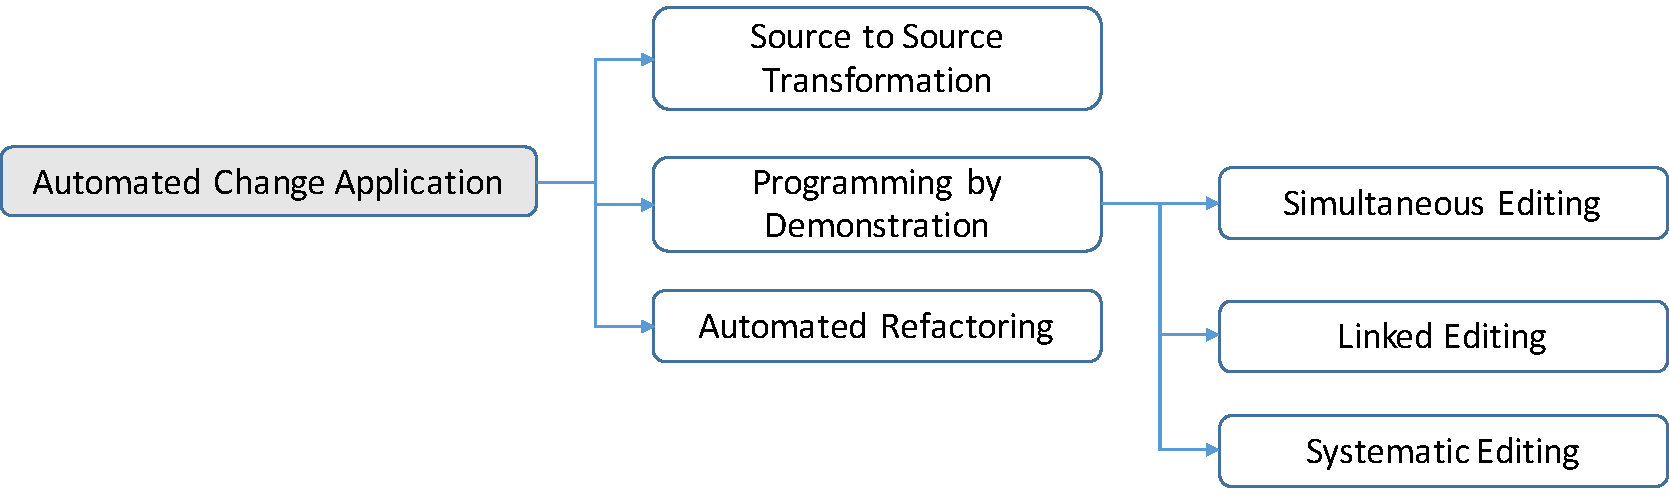
\includegraphics[width=0.95\textwidth]{images/AutomatedChange.pdf}
 \caption{Automated Change Application and Related Research Topics} 
 \label{fig:automaticapplication} 
\end{figure}


Regardless of change types, various approaches are proposed to automatically suggest program changes or reduce the manual effort of updating software. In this section, we discuss automated change application techniques including source-to-source program transformation, Programming by Demonstration (PbD), simultaneous editing, and systematic editing.

\subsubsection{Source Transformation and Languages and Tools.} 

Source transformation tools allow programmers to author their change intent in a formal syntax and automatically update a program using the change script. Most source transformation tools automate repetitive and error-prone program updates. The most ubiquitous and the least sophisticated approach to program transformation is text substitution. More sophisticated systems use program structure information. For example, A* \cite{Ladd1995} and TAWK \cite{Griswold1996} expose syntax trees and primitive data structures. Stratego/XT is based on algebraic data types and term pattern matching\cite{Visser2004}. These tools are difficult to use as they require programmers to understand low-level program representations. TXL attempts to hide these low-level details by using an extended syntax of the underlying programming language~\cite{Cordy2006}. Boshernitsan et al.'s iXJ enables programmers to perform systematic code transformations easily by providing a visual language and a tool for describing and prototyping source transformations. Their user study shows that iXj's visual language is aligned with programmers' mental model of code changing tasks~\cite{Boshernitsan2007}. Coccinelle \cite{Padioleau2008:auto} allows programmers to safely apply crosscutting updates to Linux device drivers. We describe two seminal approaches with more details. 
%Erwig and Ren \cite{Erwig2002} designed a rule-based language to express systematic updates in Haskell. 

\paragraph{\textbf{Example: TXL}} TXL is a programming language and rapid prototyping system specifically designed to support structural source transformation. TXL's source transformation paradigm consists of parsing the input text into a structure tree, transforming the tree to create a new structure tree, and unparsing the new tree to a new output text. Source text structures to be transformed are described using an unrestricted ambiguous context free grammar in extended Backus-Nauer (BNF) form. Source transformations are described by example, using a set of context sensitive structural transformation rules from which an application strategy is automatically inferred. 

Each transformation rule specifies a {\em target type} to be transformed, a {\em pattern} (an example of the particular instance of the type that we are interested in replacing), and a {\em replacement} (an example of the result we want when we find such an instance). In particular, the pattern is an actual source text example expressed in terms of tokens (terminal symbols) and variables (non-terminal types). When the pattern is matched, variable names are bound to the corresponding instances of their types in the match. Transformation rules can be composed like function compositions.  

%As shown in Figure~\ref{fig:txl}, a typical TXL file consists of two parts. The first part defines a context-free grammar to describe program syntax, while the second part describes a set of transformation rules to manipulate the syntax. For our illustrative example, the grammar defines a simple language that only allows numbers, addition and subtraction numerical expressions. The rule \codefont{resolveAddition} describes the resolution of an addition expression by replacing the expression with a number value \codefont{N1 [ + N2 ]}. Given such a file, the TXL program transformation engine automatically transforms programs of the syntactic structure by applying the rules. TXL was used to automate various code translation tasks, like ASP-to-NSP and Java-to-C\#~\cite{Chu:08,Hassan:2005,El-Ramly:2006,Tonella:04}.

\newtext{TXL programs normally consist of three parts, a context-free “base” grammar for the language to be manipulated, a set of context-free grammatical “overrides” (extensions or changes) to the base grammar, and a rooted set of source transformation rules to implement transformation of the extensions to the base language, as shown in Figure~\ref{fig:txl}. This TXL program overrides the grammar of statements to allow a new statement form. The transformation rule {\tt main} transforms the new form of a statement {\tt V+=E} to an old statement { \tt V:= V+(E)}. In other words, if there are two statements {\tt foo+=bar} and {\tt baz+=boo} they will be transformed to {\tt foo:= foo+(bar)} and {\tt baz:=baz+(boo)} at the source code level. }

\begin{figure}
\centering
\scalebox{0.9}{
	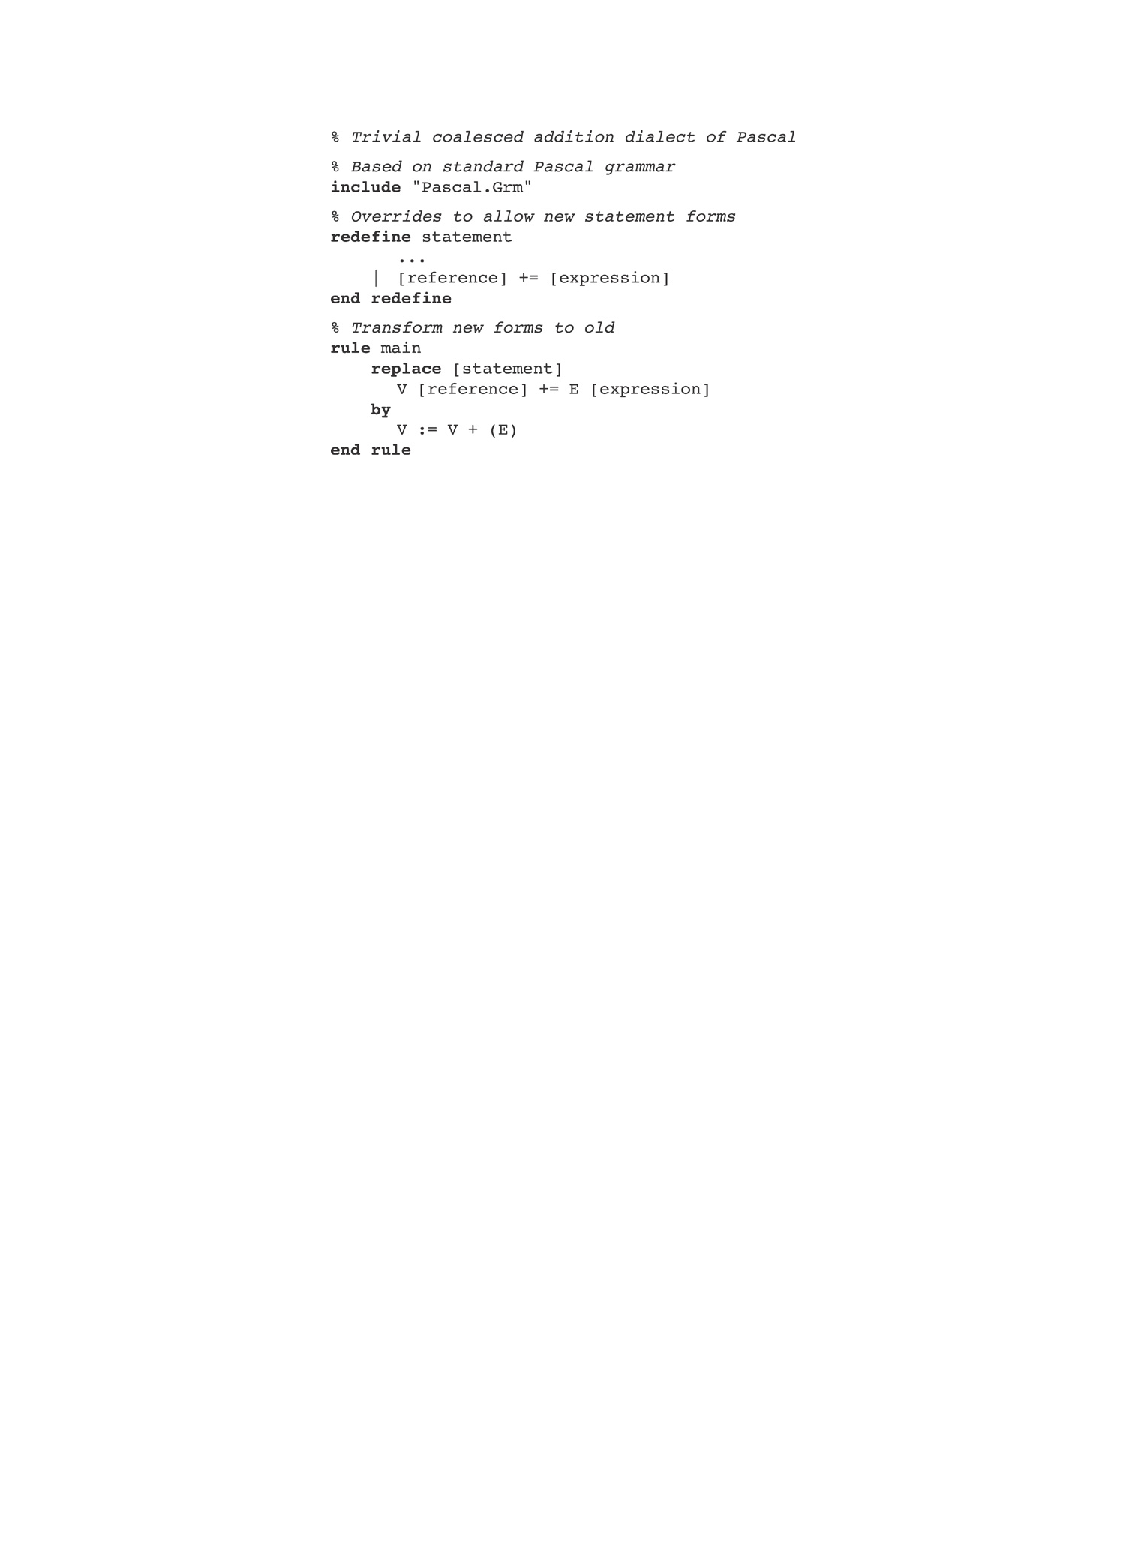
\includegraphics{images/txl2.pdf}
}
\caption{\newtext{A simple exemplar TXL file based on~\cite{txltour}}}
\label{fig:txl}
\end{figure}

\paragraph{\textbf{Example: iXj.}} 
iXj's pattern language consists of a {\em selection pattern} and a {\em transformation action}. A selection pattern is similar to our rules' antecedent, and a transformation action is similar to our rules' consequent. iXj's transformation language allows grouping of code elements using a wild-card symbol \codefont{*}. Figure \ref{ixj_example} shows an example selection pattern and a transformation pattern. 

\begin{figure} 
{\it Selection pattern}: \\
\codefont{* expression instance of java.util.Vector (:obj).removeElement(:method)(* expressions(:args))} \\
\it{Match calls to the {removeElement()} method where the {obj} expression is a subtype of {java.util.Vector}.} \\
{\it Transformation action}:\\
\codefont{\$obj\$.remove(\$obj\$.indexOf(\$args\$))} \\
\it{Replace these calls with with calls to the {remove()} method whose argument is the index of an element to remove.} 
\caption{Example iXj transformation} 
\label{ixj_example} 
\end{figure} 


To reduce the burden of learning the iXj pattern language syntax, iXj's visual editor scaffolds this process through from-example construction and iterative refinement; When a programmer selects an example code fragment to change, iXj automatically generates an initial pattern from the code selection and visualizes all code fragments matched by the initial pattern. The initial pattern is presented in a pattern editor, and a programmer can modify it interactively and see the corresponding matches in the editor. A programmer may edit the transformation action and see the preview of program updates interactively. 

\subsubsection{Programming by Demonstration.} 
Programming by Demonstration is also called Programming by Example (PbE). It is an end-user development technique for teaching a computer or a robot new behaviors by demonstrating the task to transfer directly instead of manually programming the task.  Approaches were built to generate programs based on the text-editing actions demonstrated or text change examples provided by users~\cite{Nix1984,wiki:bsd-comparison,LaH1995,LWD2001}. For instance, TELS records editing actions such as search-and-replace, and generalizes them into a program that transforms input to output~\cite{wiki:bsd-comparison}. It leverages heuristics to match actions against each other to detect any loop in the user-demonstrated program. 

SMARTedit is a representative early effort of applying PbD to text editing. It automates repetitive text-editing tasks by learning programs to perform them using techniques drawn from machine learning~\cite{LWD2001}. SMARTedit represents a text-editing program as a series of functions that alter the state of the text editor (i.e., the contents of the file, or the cursor position). Like macro recording systems, SMARTedit learns the program by observing a user performing her task. However, unlike macro recorders, SMARTedit examines the context in which the user's actions are performed and learns programs that work correctly in new contexts. Below, we describe two seminal PBD approaches applied to software engineering to automate repetitive program changes. 

\begin{figure}
\centering
\scalebox{0.5}{
	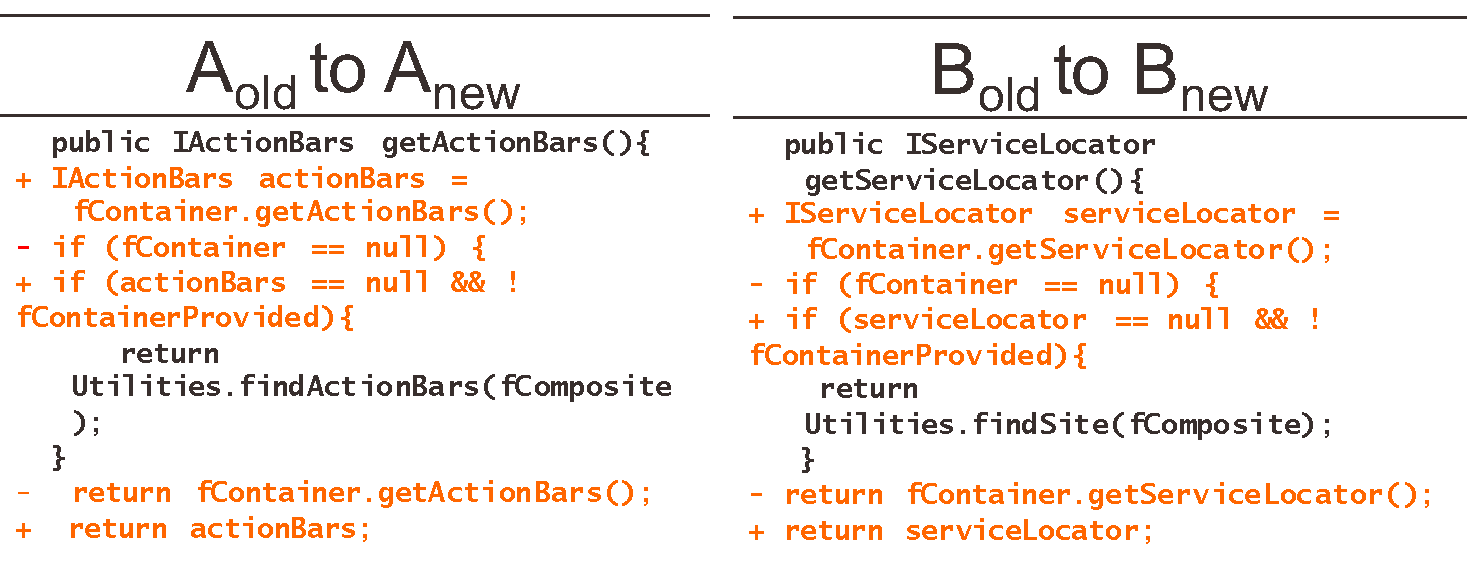
\includegraphics{images/laseexample.pdf}
}
\caption{\newtext{An example of non-contiguous, abstract edits that can be applied using LASE~\cite{Meng12:lase}}}
\label{fig:lase}
\end{figure}



\paragraph{Simultaneous Editing.}
Simultaneous editing repetitively applies source code changes that are interactively demonstrated by users~\cite{MiM2001}. When users apply their edits in one program context, the tool replicates the \emph{exact lexical} edits to other code fragments, or transforms code accordingly. Linked Editing requires users to first specify the similar code snippets which they want to modify in the same way~\cite{TBG2004}. As users interactively edit one of these snippets, Linked Editing simultaneously applies the identical edits to other snippets. 
%CloneTracker takes the output of a clone detector as input and creates a descriptor for each clone~\cite{DuR2007}. With such descriptors, CloneTracker tracks clones across program versions and identifies any modification to those clones. %Similar to Linked Editing, CloneTracker also echoes edits in one clone to other counterparts upon a developer's request. Clever is another clone management system that tracks code clone groups and detects any inconsistent change applied to clones within the same group~\cite{NNP2009}. If a clone misses the updates applied to the other clones in the same group, Clever automatically suggests the missing update to that clone.

\paragraph{Systematic Editing.} Systematic editing is the process of applying similar, but not necessarily identical, program changes to multiple code locations. High-level changes are often systematic\textemdash consisting of related transformations at a code level. In particular, crosscutting concerns, refactoring, and API update mentioned in Sections~\ref{sec:perfective},~\ref{sec:adaptive}, and~\ref{sec:preventive} are common kinds of systematic changes, because making these changes during software evolution involves tedious effort of locating individual change locations and applying similar but not identical changes. Several approaches have been proposed to infer the general program transformation from one or more code change examples provided by developers~\cite{MKM2011,Meng12:lase,Rolim:2017}, and apply the transformation to other program contexts in need of similar changes. \newtext{Specifically, LASE requires developers to provide multiple similarly changed code examples in Java (at least two)~\cite{Meng12:lase}. By extracting the commonality between demonstrated changes and abstracting the changes in terms of identifier usage and control- or data-dependency constraints in edit contexts, LASE creates a general program transformation, which can both detect code locations that should be changed similarly, and suggest customized code changes for each candidate location. For example, in Figure~\ref{fig:lase}, LASE can take the change example on from $A_{old}$ to $A_{new}$ as input and apply to the code on $B_{old}$ to generate $B_{new}$. Such change is similar but customized to the code on the right.} 


